\section{Analysis}
%
\begin{figure}%
  \def\frac{0.5}
  \begin{minipage}[b]{0.5\linewidth}
    \centering
    % Ours with and without step loss
    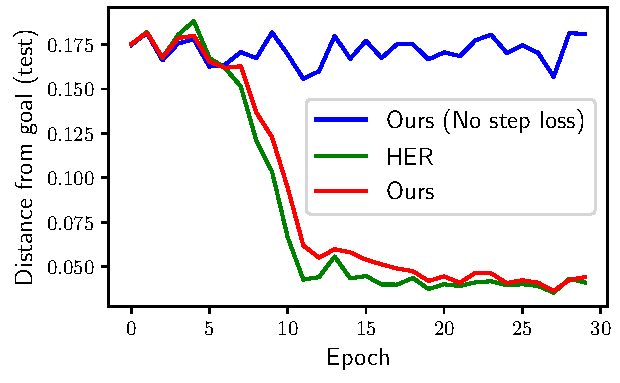
\includegraphics[width=\frac\columnwidth]{media/res/ablate-ddpg-with-without-step-loss/FetchPush-6efc1de-ddpgepoch-test/ag_g_dist.pdf}%
    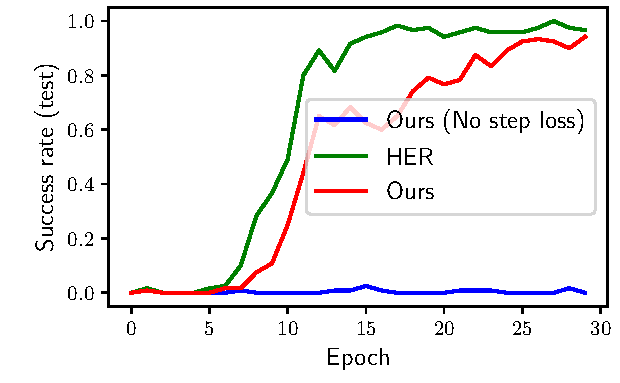
\includegraphics[width=\frac\columnwidth]{media/res/ablate-ddpg-with-without-step-loss/FetchPush-6efc1de-ddpgepoch-test/success_rate.pdf}\\
    \subcaption{Do we really need the step loss?}
    \label{fig:with-and-without-step-loss-a}
  \end{minipage}
  \begin{minipage}[b]{0.5\linewidth}
    \centering
    % Ours with and without goal rewards
    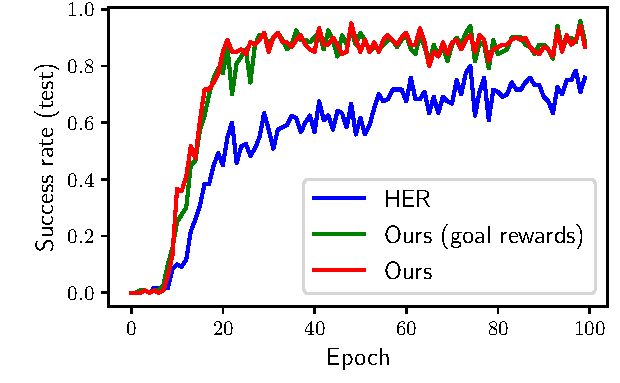
\includegraphics[width=\frac\columnwidth]{media/res/ablate-ours-with-goal-reward/FetchPickAndPlace-dqstepoch-test/success_rate.pdf}%
    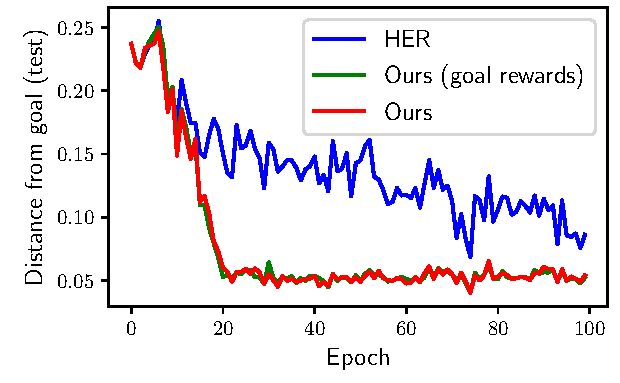
\includegraphics[width=\frac\columnwidth]{media/res/ablate-ours-with-goal-reward/FetchPickAndPlace-dqstepoch-test/ag_g_dist.pdf}\\
    \subcaption{Effect of goal-rewards}
    \label{fig:with-and-without-step-loss-b}
  \end{minipage}
  \caption{
    Effects of adding the goal-reward or removing the step-loss to our method.
    The left two plots on Fetch Push task show that the step loss is critical to the working of our
    method in the absence of goal rewards.
    The right two plots on Fetch Pick and Place task show that goal-rewards do not help much in raising the
    performance of our method. This shows that one-step loss captures the
    information that is equivalent to the providing the goal-rewards.}
  \label{fig:with-and-without-step-loss}%
\end{figure}%
% 

%
\begin{figure}%
  \def\frac{0.5}
\begin{minipage}[b]{\frac\linewidth}\centering
  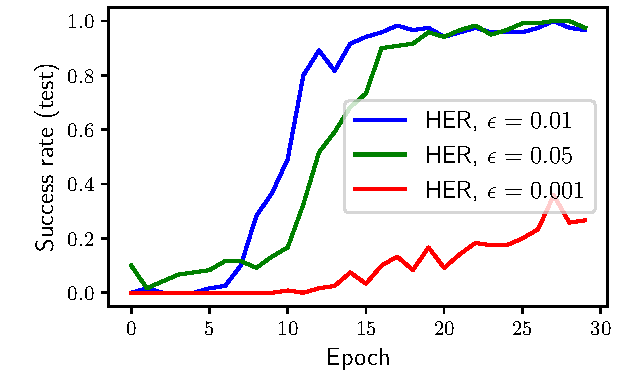
\includegraphics[width=\frac\columnwidth]{media/res/ablate-ddpg-dqst-low_tresh_chosen-low_thresh_alt-ddpg/0.05-be0910cepoch-test/success_rate.pdf}%
  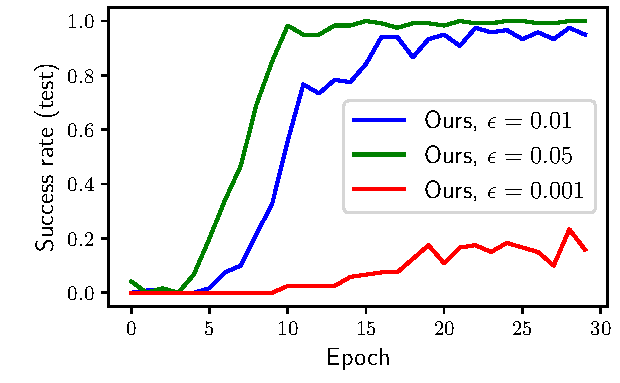
\includegraphics[width=\frac\columnwidth]{media/res/ablate-ddpg-dqst-low_tresh_chosen-low_thresh_alt-dqst/0.001-FetchPushPR-be467dfepoch-test/success_rate.pdf}%
  \subcaption{Sucesss rate}\label{fig:success-rate}
  \end{minipage}\begin{minipage}[b]{\frac\linewidth}\centering
  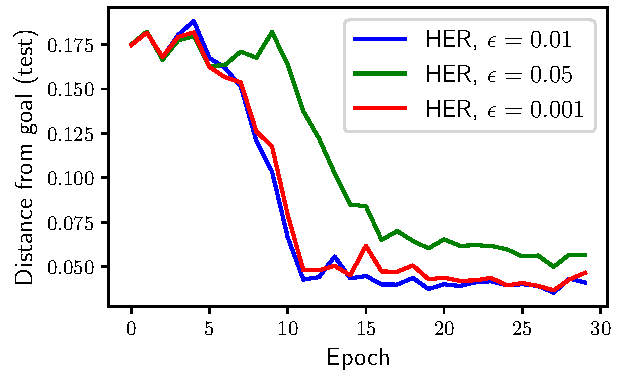
\includegraphics[width=\frac\columnwidth]{media/res/ablate-ddpg-dqst-low_tresh_chosen-low_thresh_alt-ddpg/0.05-be0910cepoch-test/ag_g_dist.pdf}%
  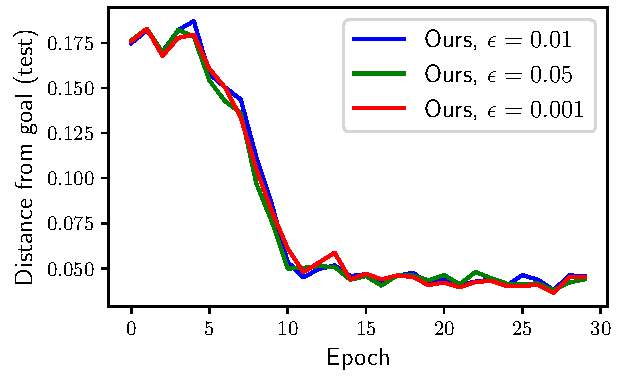
\includegraphics[width=\frac\columnwidth]{media/res/ablate-ddpg-dqst-low_tresh_chosen-low_thresh_alt-dqst/0.001-FetchPushPR-be467dfepoch-test/ag_g_dist.pdf}%
  \subcaption{Distance from goal}\label{fig:distance}
\end{minipage}
  \caption{Effects of distance threshold on HER and our method on Fetch Push
task. Although the success rate decreases as the distance threshold decreases,
the distance to the goal is not affected. For HER, the distance to the goal
reaches lower values with smaller distance thresholds.}%
  \label{fig:with-different-distance-thresholds}%
\end{figure}%
% 

To gain a deeper understanding of the method we perform three additional
experiments on different tasks. We ask the following questions:
(a) How important is the step loss?
(b) What happens the goal-reward is also available to our method?
(c) How sensitive is HER and our method to the distance-threshold?
\paragraph{How important is the step loss?}
%
We choose the Fetch-Push task for this experiment.
We run our algorithm with no goal reward and without the step loss on Fetch Push
task. Results show that our algorithm fails to reach the goal when the
step-loss is remove (Fig.~\ref{fig:with-and-without-step-loss}).

\paragraph{What happens the goal-reward is also available to our method?}
We run this experiment on the Fetch PickAndPlace task. We find that
goal-rewards do not effect the performance of our algorithm further
solidifying the avoidability of goal-reward (Fig~\ref{fig:with-and-without-step-loss}).

\paragraph{How sensitive is HER and our method to the distance-threshold?}
In the absence of goal-rewards, our algorithm is not to able capture distance
threshold information that decides whether the agent has reached the goal or
not. This information is available to HER. To understand the
sensitivity of our algorithm and HER on this parameter, we vary it over
0.05 (the original HER value), 0.01 and 0.001 meters
(Figure~\ref{fig:with-different-distance-thresholds}). Results show that
for the success-rate metric,which is itself a function of this
parameter, both algorithms affected equally. For the distance-from-goal,
only HER is affected. This fits our expectations as set up in 
section~\ref{sec:hyperparams}.




